% Options for packages loaded elsewhere
\PassOptionsToPackage{unicode}{hyperref}
\PassOptionsToPackage{hyphens}{url}
%
\documentclass[
]{article}
\usepackage{amsmath,amssymb}
\usepackage{lmodern}
\usepackage{iftex}
\ifPDFTeX
  \usepackage[T1]{fontenc}
  \usepackage[utf8]{inputenc}
  \usepackage{textcomp} % provide euro and other symbols
\else % if luatex or xetex
  \usepackage{unicode-math}
  \defaultfontfeatures{Scale=MatchLowercase}
  \defaultfontfeatures[\rmfamily]{Ligatures=TeX,Scale=1}
\fi
% Use upquote if available, for straight quotes in verbatim environments
\IfFileExists{upquote.sty}{\usepackage{upquote}}{}
\IfFileExists{microtype.sty}{% use microtype if available
  \usepackage[]{microtype}
  \UseMicrotypeSet[protrusion]{basicmath} % disable protrusion for tt fonts
}{}
\makeatletter
\@ifundefined{KOMAClassName}{% if non-KOMA class
  \IfFileExists{parskip.sty}{%
    \usepackage{parskip}
  }{% else
    \setlength{\parindent}{0pt}
    \setlength{\parskip}{6pt plus 2pt minus 1pt}}
}{% if KOMA class
  \KOMAoptions{parskip=half}}
\makeatother
\usepackage{xcolor}
\IfFileExists{xurl.sty}{\usepackage{xurl}}{} % add URL line breaks if available
\IfFileExists{bookmark.sty}{\usepackage{bookmark}}{\usepackage{hyperref}}
\hypersetup{
  pdftitle={Relatório trabalho prático 4},
  pdfauthor={César A. Galvão 19/0011572; Gabriela Carneiro 18/0120816},
  hidelinks,
  pdfcreator={LaTeX via pandoc}}
\urlstyle{same} % disable monospaced font for URLs
\usepackage[margin=1in]{geometry}
\usepackage{graphicx}
\makeatletter
\def\maxwidth{\ifdim\Gin@nat@width>\linewidth\linewidth\else\Gin@nat@width\fi}
\def\maxheight{\ifdim\Gin@nat@height>\textheight\textheight\else\Gin@nat@height\fi}
\makeatother
% Scale images if necessary, so that they will not overflow the page
% margins by default, and it is still possible to overwrite the defaults
% using explicit options in \includegraphics[width, height, ...]{}
\setkeys{Gin}{width=\maxwidth,height=\maxheight,keepaspectratio}
% Set default figure placement to htbp
\makeatletter
\def\fps@figure{htbp}
\makeatother
\setlength{\emergencystretch}{3em} % prevent overfull lines
\providecommand{\tightlist}{%
  \setlength{\itemsep}{0pt}\setlength{\parskip}{0pt}}
\setcounter{secnumdepth}{5}
\usepackage{helvet} \renewcommand\familydefault{\sfdefault}
\usepackage{booktabs}
\usepackage{longtable}
\usepackage{array}
\usepackage{multirow}
\usepackage{wrapfig}
\usepackage{float}
\usepackage{colortbl}
\usepackage{pdflscape}
\usepackage{tabu}
\usepackage{threeparttable}
\usepackage{threeparttablex}
\usepackage[normalem]{ulem}
\usepackage{makecell}
\usepackage{xcolor}
\ifLuaTeX
  \usepackage{selnolig}  % disable illegal ligatures
\fi

\title{Relatório trabalho prático 4}
\author{César A. Galvão 19/0011572 \and Gabriela Carneiro 18/0120816}
\date{10 de September de 2022}

\begin{document}
\maketitle

\newpage{}

{
\setcounter{tocdepth}{2}
\tableofcontents
}
\let\oldsection\section
\renewcommand\section{\clearpage\oldsection}

\begin{center} 

\textbf{Resumo} 

\end{center}

Nesta atividade foram implementadas em R um algoritmo EM e um método
MCMC. Para cada algoritmo, foram estimados três parâmetros:
probabilidade de o lote vir da máquina A (\(p\)) e a probabilidade de
que, dado que uma determinada peça tenha sido produzida pela máquina A
ou B, a peça seja defeituosa (\(\theta_A\), \(\theta_B\)). Por fim, são
apresentados histogramas com a função de probabilidade conjunta obtida
pelos parâmetros estimados sobreposta em formato de pontos.\footnote{Todos
  os documentos desse relatório podem ser verificados no repositório
  \url{https://github.com/cesar-galvao/Estatistica-computacional}}

\hypertarget{introduuxe7uxe3o}{%
\section{Introdução}\label{introduuxe7uxe3o}}

\hypertarget{muxe9todo}{%
\section{Método}\label{muxe9todo}}

\hypertarget{muxe9todo-em}{%
\subsection{Método EM}\label{muxe9todo-em}}

\hypertarget{amostrador-de-gibbs}{%
\subsection{Amostrador de Gibbs}\label{amostrador-de-gibbs}}

\hypertarget{resultados}{%
\section{Resultados}\label{resultados}}

Para o método EM, obteve-se a seguinte estimativa final para os
parâmetros ao final de 29 iterações:

\begin{longtable}{ccc}
\toprule
$\theta_A$ & $\theta_B$ & $p$\\
\midrule
\endfirsthead
\multicolumn{3}{@{}l}{\textit{(continued)}}\\
\toprule
$\theta_A$ & $\theta_B$ & $p$\\
\midrule
\endhead

\endfoot
\bottomrule
\endlastfoot
\cellcolor{gray!15}{0.0517882} & \cellcolor{gray!15}{0.0905156} & \cellcolor{gray!15}{0.6908754}\\*
\end{longtable}

A função de distribuição conjunta, com os parâmetros obtidos pelo
algoritmo EM, é

\begin{align}
  P(y) = (1-p)P(y|\theta_A) + p P(y|\theta_B).
\end{align}

Além disso, obteve-se o seguinte histograma com a função de distribuição
conjunta, representada por pontos:

\begin{figure}

{\centering 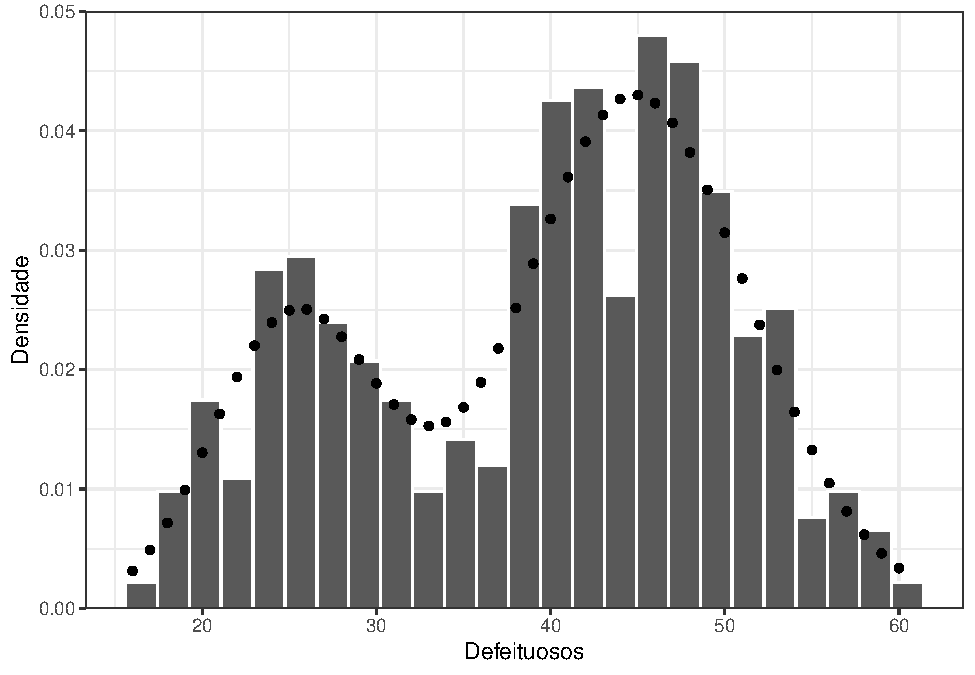
\includegraphics[width=0.6\linewidth]{relatorio_tp4_files/figure-latex/histograma-EM-1} 

}

\caption{Histograma de da amostra e função de distribuição conjunta com parâmetros obtidos pelo algoritmo EM.}\label{fig:histograma-EM}
\end{figure}

\hypertarget{anexo-a---cuxf3digo-comentado}{%
\section*{Anexo A - código
comentado}\label{anexo-a---cuxf3digo-comentado}}
\addcontentsline{toc}{section}{Anexo A - código comentado}

\end{document}
